\documentclass[12pt,fleqn]{article}
\usepackage{greg}
\usepackage[baskerville,vvarbb]{newtxmath}
\usepackage{fontspec}
\usepackage{titlesec}
\usepackage{titling}
\usepackage[nottoc]{tocbibind}
\usepackage{fancyvrb}
\setmainfont{Baskerville}
\setsansfont{Quadrat-Serial}
\setmonofont{Courier New}
\urlstyle{rm}

\renewenvironment{abstract}{\section*{\abstractname}}{}
\titleformat*{\section}{\large\sffamily}
\titleformat*{\subsection}{\normalsize\sffamily}
\titleformat*{\subsubsection}{\normalsize\sffamily}
\titleformat{\chapter}[hang]{\LARGE\sffamily}{\LARGE\thechapter}{1ex}{}[]
\titleformat{name=\chapter,numberless}[hang]{\LARGE\sffamily}{}{0ex}{}[]
\renewcommand{\maketitlehooka}{\large\sffamily}

\title{Discrete differential geometry in homotopy type theory}
\author{Greg Langmead}
\begin{document}

\maketitle

\begin{abstract}
Homotopy type theory captures all the major concepts of differential geometry including forms, connections, curvature, and gauge theory. We show this by focusing on combinatorial manifolds, which are discrete in the sense of real cohesion\cite{shulman_cohesion}, and drawing inspiration from the similarly young field of discrete differential geometry.

\end{abstract}

\begin{quote} 
\centering
``It is always ourselves we work on, whether we realize it or not. There is no other work to be done in the world.'' --- Stephen Talbott, \emph{The Future Does Not Compute}\cite{talbott}
\end{quote}

\section{Introduction: Discrete differential geometry}

The observation that sparks the following discussion is this: if we can manage to reformulate differential geometry in discrete terms (i.e. finite, without infinitesimals) then we may also be able to construct it synthetically in homotopy type theory. Furthermore, if we do capture geometry in HoTT then there's a chance that it can become clearer and smaller. We would then have new tools, a new audience, and a new program to (re)explore geometry, gauge theory, low dimensional topology, and mathematical physics.

Applied mathematicians and computer scientists have been developing discrete differential geometry (DDG) for many years. The 2003 Ph.D. thesis of Anil Hirani \cite{hiranidec} (see also the multi-author follow-up \cite{desbrundec}) defines finite versions of vector fields, differential forms, the wedge product, the Hodge star, and several differential operators (exterior derivative, div, grad, curl, Laplace-Beltrami, Lie derivative). Hirani and others cite Whitney's 1957 book \emph{Geometric Integration Theory}\cite{whitney1957} which develops a theory of cochains by integrating smooth forms over chains. In 2004 Melvil Leok, Jerrold Marsden, and Alan Weinstein \cite{leok} defined discrete connections on principal bundles. This is probably the work most spiritually similar to this paper. The motivation for the above constructions was applied mathematics: modeling the differential equations of mechanics and fluid mechanics with the so-called ``finite element'' methods. The theory has been adopted and extended by the computer graphics community as well (see Keenan Crane's course notes \cite{crane_ddg} for a gentle survey).

The applied category theory community has begun to develop category theoretic foundations and software libraries to increase the reusability and compositionality of finite element methods in science and engineering problems. See for example recent work to bring discrete exterior calculus into the AlgebraicJulia library \cite{morris_decapodes} \cite{patterson_diffeq}.

For these classically-minded applied mathematicians DDG is defined on combinatorial manifolds such as simplicial complexes, of any finite dimension. The 0-cells play the role of points, the 1-cells are path segments, and so on. They define \( n \)-forms as functions on the \( n \)-dimensional faces of the manifold into the real numbers, which is then extended by linearity to arbitrary \( n \)-chains. Exterior differentiation is defined by Stokes theorem (which is no longer a theorem in this setting), by which we mean the following. 

\begin{mydef}
(Exterior derivative in DDG.) Let \( \omega \) be an \( n-1 \)-form on a combinatorial manifold \( M \), and let \( \Omega \) be an \( n \)-face of \( M \). Let \( \partial \) be the boundary operator on faces. The exterior derivative \( d \) is defined by 
\[ 
 d\omega(\Omega) = \omega(\partial\Omega).
\]
\end{mydef}

We will take the following path. We will use DDG as a stepping stone between smooth geometry and HoTT. We will learn how to see the finite analogues of infinitesimal constructions, and then use the syntax of type theory to re-present them. It won't always be a two-step process! Sometimes even the smooth arguments are made with finite combinatorial methods, and then a limit is taken. This is especially true where the Gauss-Bonnet and Poincaré-Hopf theorems are concerned.
\[\mathrm{Differential\ geometry}\longrightarrow\mathrm{Discrete\ differential\ geometry}\longrightarrow \mathrm{Homotopy\ type\ theory}\]


\section{Examples}
\subsection{The tangent bundle of the 2-sphere}

We will define some higher inductive types to serve as domain and codomain of these motivating examples.

First we need a square, which will be a stand-in for a circle that can support a notion of a quarter-rotation. 

\begin{mydef}
The higher inductive type \( C_4 \) (where C stands for ``circle'').
\begin{align*}
C_4 &: \Type \\
c_1, c_2, c_3, c_4 &: C_4 \\
c_1c_2 &: c_1 = c_2 \\
c_2c_3 &: c_2 = c_3 \\
c_3c_4 &: c_3 = c_4 \\
c_4c_1 &: c_4 = c_1 \\
\end{align*}
\end{mydef}

\begin{tikzpicture}[
node distance = 15mm and 15mm,
V/.style = {circle, fill, draw=black, inner sep=1pt, font=\footnotesize},
every edge quotes/.style = {auto, font=\footnotesize},
arrow/.style={->,semithick}
]
\begin{scope}[nodes=V]
  \node[label=above left:\( c_1 \)] (1) {};
  \node[label=above right:\( c_2 \)] (2) [right=of 1]  {};
  \node[label=below right:\( c_3 \)] (3) [below=of 2]  {};
  \node[label=below left:\( c_4 \)] (4) [below=of 1]  {};
\end{scope}
\draw[arrow]
        (1)  edge["\( c_1c_2 \)"] (2)
        (2)  edge["\( c_2c_3 \)"] (3)
        (3)  edge["\( c_3c_4 \)"] (4)
        (4)  edge["\( c_4c_1 \)"] (1);
\end{tikzpicture}


We may also think of \( C_4 \) as the join of the two-element sets \( \{c_1, c_3\}* \{c_2, c_4\} \).

\begin{mydef}
The HIT \( \oo_0 \) is just 6 points, intended as the 0-skeleton of an octahedron, with vertices named after the colors on the faces of a Rubik's Cube.
\[ w, y, b, r, g, o : \oo_0 \]
\end{mydef}

\begin{mydef}
The HIT \( \oo_1 \) is the 1-skeleton of an octahedron.
\begin{align*}
w, y, b, r, g, o &: \oo_1 \\
wb &: w=b \\
wr &: w=r \\
wg &: w=g \\
wo &: w=o \\
yb &: y=b \\
yr &: y=r \\
yg &: y=g \\
yo &: y=o \\
br &: b=r \\
rg &: r=g \\
go &: g=o \\
ob &: o=b 
\end{align*}
\end{mydef}

\begin{mydef}
The HIT \( \oo \) which has 8 faces:
\begin{align*}
w, y, b, r, g, o &: \oo \\
wb &: w=b \\
wr &: w=r \\
wg &: w=g \\
wo &: w=o \\
yb &: y=b \\
yr &: y=r \\
yg &: y=g \\
yo &: y=o \\
br &: b=r \\
rg &: r=g \\
go &: g=o \\
ob &: o=b \\
wbr &: wb\cdot br\cdot wr^{-1} = \refl_w \\
wrg &: wr\cdot rg\cdot wg^{-1} = \refl_w \\
wgo &: wg\cdot go\cdot wo^{-1} = \refl_w \\
wob &: wo\cdot ob\cdot wb^{-1} = \refl_w \\
yrb &: yr\cdot rb\cdot yb^{-1} = \refl_y \\
ygr &: yg\cdot gr\cdot yr^{-1} = \refl_y \\
yog &: yo\cdot og\cdot yg^{-1} = \refl_y \\
ybo &: yb\cdot bo\cdot yo^{-1} = \refl_y
\end{align*}
\end{mydef}

\begin{figure}[h]
\centering
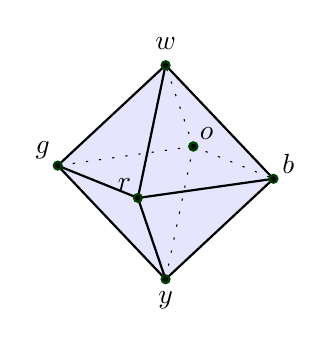
\begin{tikzpicture}%
  [x={(-0.860769cm, -0.121512cm)},
  y={(0.508996cm, -0.205391cm)},
  z={(-0.000053cm, 0.971107cm)},
  scale=1,
  back/.style={loosely dotted, thin},
  edge/.style={black, thick},
  facet/.style={fill=blue!95!black,fill opacity=0.1},
  vertex/.style={inner sep=1pt,circle,draw=green!25!black,fill=black,thick}]
\coordinate (-1, -1, 0) at (-1, -1, 0);
\coordinate (-1, 1, 0) at (-1, 1, 0);
\coordinate (0, 0, -1) at (0, 0, -1);
\coordinate (0, 0, 1) at (0, 0, 1);
\coordinate (1, -1, 0) at (1, -1, 0);
\coordinate (1, 1, 0) at (1, 1, 0);
%% Drawing edges in the back
%%
\draw[edge,back] (-1, -1, 0) -- (-1, 1, 0);
\draw[edge,back] (-1, -1, 0) -- (0, 0, -1.4);
\draw[edge,back] (-1, -1, 0) -- (0, 0, 1.4);
\draw[edge,back] (-1, -1, 0) -- (1, -1, 0);
%% Drawing vertices in the back
%%
\node[vertex] at (-1, -1, 0)     {};
%% Drawing the facets
%%
\fill[facet] (1, 1, 0) -- (0, 0, -1.4) -- (1, -1, 0) -- cycle {};
\fill[facet] (1, 1, 0) -- (0, 0, 1.4) -- (1, -1, 0) -- cycle {};
\fill[facet] (1, 1, 0) -- (-1, 1, 0) -- (0, 0, 1.4) -- cycle {};
\fill[facet] (1, 1, 0) -- (-1, 1, 0) -- (0, 0, -1.4) -- cycle {};
%% Drawing edges in the front
%%
\draw[edge] (-1, 1, 0) -- (0, 0, -1.4);
\draw[edge] (-1, 1, 0) -- (0, 0, 1.4);
\draw[edge] (-1, 1, 0) -- (1, 1, 0);
\draw[edge] (0, 0, -1.4) -- (1, -1, 0);
\draw[edge] (0, 0, -1.4) -- (1, 1, 0);
\draw[edge] (0, 0, 1.4) -- (1, -1, 0);
\draw[edge] (0, 0, 1.4) -- (1, 1, 0);
\draw[edge] (1, -1, 0) -- (1, 1, 0);
%% Drawing the vertices in the front
%%
\begin{scope}[nodes=vertex]
\node[label=above right:\( b \)] at (-1, 1, 0)     {};
\node[label=below:\( y \)] at (0, 0, -1.4)     {};
\node[label=above:\( w \)] at (0, 0, 1.4)     {};
\node[label=above left:\( g \)] at (1, -1, 0)     {};
\node[label=above left:\( r \)] at (1, 1, 0)     {};
\node[label=above right:\( o \)] at (-1, -1, 0)     {};
\end{scope}
\end{tikzpicture}
\caption{The HIT \( \oo \) which has 6 points, 12 1-paths, 8 2-paths.}
\end{figure}


We have obvious maps \( \oo_0\xrightarrow[]{i_0} \oo_1\xrightarrow[]{i_1} \oo \) that include each skeleton into the next-higher-dimensional skeleton.

Combinatorial spaces have a concept called the \emph{link} of a vertex, which will be the main tool by which we connect with manifold theory. The vertices in the link are the vertices that are one edge away from the given point, and the edges in the link are the edges connecting these. If the link of an \( n \)-dimensional combinatorial space is always a combinatorial \( n-1 \)-sphere, then we say the space is a \emph{combinatorial triangulation}. We will look only at HITs that have a link that is merely equivalent to \( C_4 \).

\begin{mydef}
If we have \( X:\Type \) then we define \( \BAut X\defeq \sit{Y:\Type} ||X=Y||_{-1} \). 
\end{mydef}

Denote by \( abcd:\BAut C_4 \) the HIT with vertices \( a, b, c, d \) and edges \( ab, bc, cd, da \) which clearly has various isomorphisms with \( C_4 \).

We can now define \( \link \) on the 0-skeleton. Extending this later on to the 1-skeleton and 2-skeleton will take us into differential geometry!

\begin{mydef}
\( \link:\oo_0\to\BAut C_4 \) is given by induction:
\begin{align*}
\link(w) &= brgo \\
\link(y) &= bogr \\
\link(b) &= woyr \\
\link(r) &= wbyg \\
\link(g) &= wryo \\
\link(o) &= wgyb
\end{align*}
We chose these orderings for the vertices by standing at the given vertex and enumerating the link in clockwise order, starting from \( w \) if possible, else \( b \).
\end{mydef}

Besides the link we also want to consider the 5-pointed object that includes the vertex itself and the edges connecting it to the vertices in the link. We will call such a shape an \emph{xbox} since it is a square with both diagonals. We will denote xboxes by extending the square notation with a fifth letter to indicate the center of the xbox. For example, we can define an xbox \( C_4c \) as follows:

\begin{mydef}
The higher inductive type \( C_4c \) with center \( c \), also denoted \( c_1c_2c_3c_4c \).
\begin{align*}
C_4c &: \Type \\
c_1, c_2, c_3, c_4, c &: C_4c \\
c_1c_2 &: c_1 = c_2 \\
c_2c_3 &: c_2 = c_3 \\
c_3c_4 &: c_3 = c_4 \\
c_4c_1 &: c_4 = c_1 \\
c_1c &: c_1 = c \\
c_2c &: c_2 = c \\
c_3c &: c_3 = c \\
c_4c &: c_4 = c 
\end{align*}
\end{mydef}

We can map our octahedron into the space of xboxes:
\begin{mydef}
\( \xbox:\oo_0\to\BAut C_4c \) is given by induction:
\begin{align*}
\xbox(w) &= brgow \\
\xbox(y) &= bogry \\
\xbox(b) &= woyrb \\
\xbox(r) &= wbygr \\
\xbox(g) &= wryog \\
\xbox(o) &= wgybo
\end{align*}
\end{mydef}

Finally we want to consider the 2-type that fills in the faces of the xbox. This is a contractible type we will call a \emph{disk}.

\begin{mydef}
The higher inductive type \( C_{4\disk} \) with center \( c \), also denoted \( c_1c_2c_3c_4c_\disk \).
\begin{align*}
C_{4\disk} &: \Type \\
c_1, c_2, c_3, c_4, c &: C_{4\disk} \\
c_1c_2 &: c_1 = c_2 \\
c_2c_3 &: c_2 = c_3 \\
c_3c_4 &: c_3 = c_4 \\
c_4c_1 &: c_4 = c_1 \\
c_1c &: c_1 = c \\
c_2c &: c_2 = c \\
c_3c &: c_3 = c \\
c_4c &: c_4 = c \\
c_1c_2c &: c_1c_2\cdot c_2c\cdot c_1c^{-1} = \refl \\
c_2c_3c &: c_2c_2\cdot c_3c\cdot c_2c^{-1} = \refl \\
c_3c_4c &: c_3c_2\cdot c_4c\cdot c_3c^{-1} = \refl \\
c_4c_1c &: c_4c_2\cdot c_1c\cdot c_4c^{-1} = \refl
\end{align*}
\end{mydef}

And we can map the octahedron into the space of disks:

\begin{mydef}
\( \disk:\oo_0\to\BAut C_{4\disk} \) is given by induction:
\begin{align*}
\xbox(w) &= brgow_\disk \\
\xbox(y) &= bogry_\disk \\
\xbox(b) &= woyrb_\disk \\
\xbox(r) &= wbygr_\disk \\
\xbox(g) &= wryog_\disk \\
\xbox(o) &= wgybo_\disk
\end{align*}
\end{mydef}

The idea of such combinatorial manifolds is that each point has a designated local disk and local sphere (and xbox) in the same way that a smooth manifold has an atlas. We want to proceed now to define bundles on this manifold. In HoTT that means constructing a map to a classifying space. The \( \link \) map will be our map, but we have only defined it on \( \oo_0 \).

Extending \( \link \) to the 1-skeleton requires new choices. We will choose a map inspired by the tangent bundle of the sphere, using the transport we can intuitively see through the embedding of \( \oo \) in 3-dimensional space as in our pictures. If you focus for a moment just on a path \( w\to b\to r \) and imagine rigidly tipping a moving equator along with a moving point, you can imagine a moving-equator point that starts at \( r \) and stays fixed when the north pole slides from \( w \) to \( b \). When the north pole continues sliding from \( b \) to \( r \) the moving-equator point moves to \( g \). Then it remains fixed when the north pole slides from \( r \) up to \( w \). So all in all we ``moved \( r \) to \( g \).'' When we track all the points on the original \( w \)-equator we see that we performed the rotation we earlier named \( R \).

\begin{figure}[h]
\centering
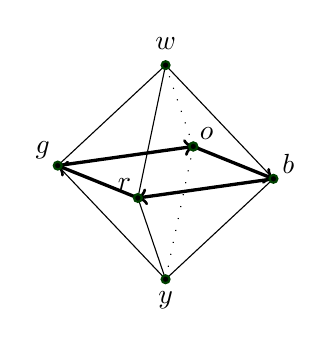
\begin{tikzpicture}%
  [x={(-0.860769cm, -0.121512cm)},
  y={(0.508996cm, -0.205391cm)},
  z={(-0.000053cm, 0.971107cm)},
  scale=1,
  eqback/.style={->, very thick},
  back/.style={loosely dotted, thin},
  eqedge/.style={->, very thick},
  edge/.style={black, thin},
  facet/.style={fill=blue!95!black,fill opacity=0.0},
  vertex/.style={inner sep=1pt,circle,draw=green!25!black,fill=black,thick}]
\coordinate (-1, -1, 0) at (-1, -1, 0);
\coordinate (-1, 1, 0) at (-1, 1, 0);
\coordinate (0, 0, -1) at (0, 0, -1);
\coordinate (0, 0, 1) at (0, 0, 1);
\coordinate (1, -1, 0) at (1, -1, 0);
\coordinate (1, 1, 0) at (1, 1, 0);
%% Drawing edges in the back
%%
\draw[edge,eqback] (-1, -1, 0) -- (-1, 1, 0);
\draw[edge,back] (-1, -1, 0) -- (0, 0, -1.4);
\draw[edge,back] (-1, -1, 0) -- (0, 0, 1.4);
\draw[edge,eqback] (1, -1, 0) -- (-1, -1, 0);
%% Drawing vertices in the back
%%
\node[vertex] at (-1, -1, 0)     {};
%% Drawing the facets
%%
\fill[facet] (1, 1, 0) -- (0, 0, -1.4) -- (1, -1, 0) -- cycle {};
\fill[facet] (1, 1, 0) -- (0, 0, 1.4) -- (1, -1, 0) -- cycle {};
\fill[facet] (1, 1, 0) -- (-1, 1, 0) -- (0, 0, 1.4) -- cycle {};
\fill[facet] (1, 1, 0) -- (-1, 1, 0) -- (0, 0, -1.4) -- cycle {};
%% Drawing edges in the front
%%
\draw[edge] (-1, 1, 0) -- (0, 0, -1.4);
\draw[edge] (-1, 1, 0) -- (0, 0, 1.4);
\draw[eqedge] (-1, 1, 0) -- (1, 1, 0);
\draw[edge] (0, 0, -1.4) -- (1, -1, 0);
\draw[edge] (0, 0, -1.4) -- (1, 1, 0);
\draw[edge] (0, 0, 1.4) -- (1, -1, 0);
\draw[edge] (0, 0, 1.4) -- (1, 1, 0);
\draw[eqedge] (1, 1, 0) -- (1, -1, 0);
%% Drawing the vertices in the front
%%
\begin{scope}[nodes=vertex]
\node[label=above right:\( b \)] at (-1, 1, 0)     {};
\node[label=below:\( y \)] at (0, 0, -1.4)     {};
\node[label=above:\( w \)] at (0, 0, 1.4)     {};
\node[label=above left:\( g \)] at (1, -1, 0)     {};
\node[label=above left:\( r \)] at (1, 1, 0)     {};
\node[label=above right:\( o \)] at (-1, -1, 0)     {};
\end{scope}
\end{tikzpicture}

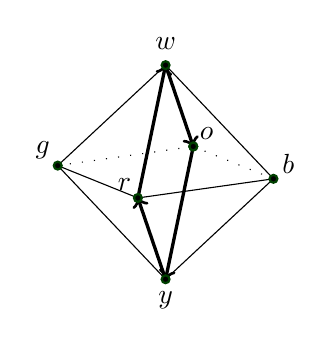
\begin{tikzpicture}%
  [x={(-0.860769cm, -0.121512cm)},
  y={(0.508996cm, -0.205391cm)},
  z={(-0.000053cm, 0.971107cm)},
  scale=1,
  eqback/.style={->, very thick},
  back/.style={loosely dotted, thin},
  eqedge/.style={->, very thick},
  edge/.style={black, thin},
  facet/.style={fill=blue!95!black,fill opacity=0.0},
  vertex/.style={inner sep=1pt,circle,draw=green!25!black,fill=black,thick}]
\coordinate (-1, -1, 0) at (-1, -1, 0);
\coordinate (-1, 1, 0) at (-1, 1, 0);
\coordinate (0, 0, -1) at (0, 0, -1);
\coordinate (0, 0, 1) at (0, 0, 1);
\coordinate (1, -1, 0) at (1, -1, 0);
\coordinate (1, 1, 0) at (1, 1, 0);
%% Drawing edges in the back
%%
\draw[edge,back] (-1, -1, 0) -- (-1, 1, 0);
\draw[edge,eqback] (-1, -1, 0) -- (0, 0, -1.4);
\draw[edge,eqback] (0, 0, 1.4) -- (-1, -1, 0);
\draw[edge,back] (1, -1, 0) -- (-1, -1, 0);
%% Drawing vertices in the back
%%
\node[vertex] at (-1, -1, 0)     {};
%% Drawing the facets
%%
\fill[facet] (1, 1, 0) -- (0, 0, -1.4) -- (1, -1, 0) -- cycle {};
\fill[facet] (1, 1, 0) -- (0, 0, 1.4) -- (1, -1, 0) -- cycle {};
\fill[facet] (1, 1, 0) -- (-1, 1, 0) -- (0, 0, 1.4) -- cycle {};
\fill[facet] (1, 1, 0) -- (-1, 1, 0) -- (0, 0, -1.4) -- cycle {};
%% Drawing edges in the front
%%
\draw[edge] (-1, 1, 0) -- (0, 0, -1.4);
\draw[edge] (-1, 1, 0) -- (0, 0, 1.4);
\draw[edge] (-1, 1, 0) -- (1, 1, 0);
\draw[edge] (0, 0, -1.4) -- (1, -1, 0);
\draw[eqedge] (0, 0, -1.4) -- (1, 1, 0);
\draw[edge] (0, 0, 1.4) -- (1, -1, 0);
\draw[eqedge] (1, 1, 0) -- (0, 0, 1.4) ;
\draw[edge] (1, 1, 0) -- (1, -1, 0);
%% Drawing the vertices in the front
%%
\begin{scope}[nodes=vertex]
\node[label=above right:\( b \)] at (-1, 1, 0)     {};
\node[label=below:\( y \)] at (0, 0, -1.4)     {};
\node[label=above:\( w \)] at (0, 0, 1.4)     {};
\node[label=above left:\( g \)] at (1, -1, 0)     {};
\node[label=above left:\( r \)] at (1, 1, 0)     {};
\node[label=above right:\( o \)] at (-1, -1, 0)     {};
\end{scope}
\end{tikzpicture}

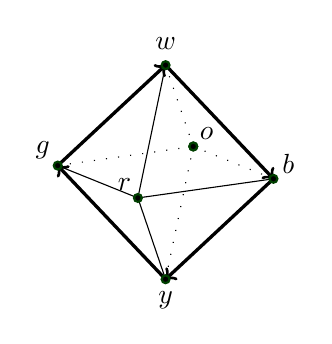
\begin{tikzpicture}%
  [x={(-0.860769cm, -0.121512cm)},
  y={(0.508996cm, -0.205391cm)},
  z={(-0.000053cm, 0.971107cm)},
  scale=1,
  eqback/.style={->, very thick},
  back/.style={loosely dotted, thin},
  eqedge/.style={->, very thick},
  edge/.style={black, thin},
  facet/.style={fill=blue!95!black,fill opacity=0.0},
  vertex/.style={inner sep=1pt,circle,draw=green!25!black,fill=black,thick}]
\coordinate (-1, -1, 0) at (-1, -1, 0);
\coordinate (-1, 1, 0) at (-1, 1, 0);
\coordinate (0, 0, -1) at (0, 0, -1);
\coordinate (0, 0, 1) at (0, 0, 1);
\coordinate (1, -1, 0) at (1, -1, 0);
\coordinate (1, 1, 0) at (1, 1, 0);
%% Drawing edges in the back
%%
\draw[edge,back] (-1, -1, 0) -- (-1, 1, 0);
\draw[edge,back] (-1, -1, 0) -- (0, 0, -1.4);
\draw[edge,back] (-1, -1, 0) -- (0, 0, 1.4);
\draw[edge,back] (1, -1, 0) -- (-1, -1, 0);
%% Drawing vertices in the back
%%
\node[vertex] at (-1, -1, 0)     {};
%% Drawing the facets
%%
\fill[facet] (1, 1, 0) -- (0, 0, -1.4) -- (1, -1, 0) -- cycle {};
\fill[facet] (1, 1, 0) -- (0, 0, 1.4) -- (1, -1, 0) -- cycle {};
\fill[facet] (1, 1, 0) -- (-1, 1, 0) -- (0, 0, 1.4) -- cycle {};
\fill[facet] (1, 1, 0) -- (-1, 1, 0) -- (0, 0, -1.4) -- cycle {};
%% Drawing edges in the front
%%
\draw[eqedge] (-1, 1, 0) -- (0, 0, -1.4);
\draw[eqedge] (0, 0, 1.4) -- (-1, 1, 0);
\draw[edge] (-1, 1, 0) -- (1, 1, 0);
\draw[eqedge] (0, 0, -1.4) -- (1, -1, 0);
\draw[edge] (0, 0, -1.4) -- (1, 1, 0);
\draw[eqedge] (1, -1, 0) -- (0, 0, 1.4);
\draw[edge] (0, 0, 1.4) -- (1, 1, 0);
\draw[edge] (1, 1, 0) -- (1, -1, 0);
%% Drawing the vertices in the front
%%
\begin{scope}[nodes=vertex]
\node[label=above right:\( b \)] at (-1, 1, 0)     {};
\node[label=below:\( y \)] at (0, 0, -1.4)     {};
\node[label=above:\( w \)] at (0, 0, 1.4)     {};
\node[label=above left:\( g \)] at (1, -1, 0)     {};
\node[label=above left:\( r \)] at (1, 1, 0)     {};
\node[label=above right:\( o \)] at (-1, -1, 0)     {};
\end{scope}
\end{tikzpicture}
\caption{The equators for \( w, b, r \).}
\end{figure}

In general we have:
\begin{mydef}
Define \( T_1:\oo\to\BAutoso \) on just the 1-skeleton by extending \( T_0 \) as follows:
Transport away from \( w \):
\begin{itemize}
\item \( T_1(wb):[b, r, g, o]\mapsto [y, r, w, o] \) (\( r, o \) fixed)
\item \( T_1(wr):[b, r, g, o]\mapsto [b, y, g, w] \) (\( b, g \) fixed)
\item \( T_1(wg):[b, r, g, o]\mapsto [w, r, y, o] \)
\item \( T_1(wo):[b, r, g, o]\mapsto [b, w, g, y] \)
\end{itemize}
Transport away from \( y \):
\begin{itemize}
\item \( T_1(yb):[b, o, g, r]\mapsto [w, o, y, r] \)
\item \( T_1(yr):[b, o, g, r]\mapsto [b, y, g, w] \)
\item \( T_1(yg):[b, o, g, r]\mapsto [y, o, w, r] \)
\item \( T_1(yo):[b, o, g, r]\mapsto [b, w, g, y] \)
\end{itemize}
Transport along the equator:
\begin{itemize}
\item \( T_1(br):[w, o, y, r]\mapsto [w, b, y, g] \) 
\item \( T_1(rg):[w, b, y, g]\mapsto [w, r, y, o] \)
\item \( T_1(go):[w, r, y, o]\mapsto [w, g, y, b] \)
\item \( T_1(ob):[w, g, y, b]\mapsto [w, o, y, r] \)
\end{itemize}
\end{mydef}

At this point we have defined a map on the 1-skeleton of \( \oo \).

\begin{myclaim}
\( T_1 \) defines a principal circle bundle with connection over the 1-skeleton of \( \oo \).
\end{myclaim}

We now want to extend this map to all of \( \oo \) by providing values for the eight faces. Here we will be guided by the classical relationship between a connection and its curvature. The curvature is computed from the connection, it doesn't contain any new data. Classically the integral of curvature over a 2-cell is the holonomy given by transport around the boundary. 

\begin{mydef}
Define \( T_2:\oo\to\BAutoso \) by extending \( T_1 \) as follows. We will send every clockwise triangle to \( R' \), the homotopy from \( \refl \) to \( R \):
\begin{itemize}
\item \( T_2(wbr)=R' \) 
\item \( T_2(wrg)=R' \)
\item \( T_2(wgo)=R' \)
\item \( T_2(ybo)=R' \)
\item \( T_2(yrb)=R' \) 
\item \( T_2(ygr)=R' \)
\item \( T_2(yog)=R' \)
\item \( T_2(ybo)=R' \)
\end{itemize}
\end{mydef}


\subsection{Combinatorial manifolds}

(This section is not quite off the ground.)

The combinatorial structure we have in mind is a nerve of a good open cover. What do we know about which smooth manifolds have such covers? While we're at it, let's survey all the combinatorial-flavored spaces and survey what smooth manifolds are homotopy equivalent to which structures.

What topological manifolds are equivalent to a CW complex? The answer is the composition of a few results summarized by Allen Hatcher\footnote{\url{https://mathoverflow.net/questions/201944/topological-n-manifolds-have-the-homotopy-type-of-n-dimensional-cw-complexes}} (citing \cite{kirby_siebenmann} and \cite{freedman_quinn}):

\begin{quote}
Every topological manifold has a handlebody structure except in dimension 4, where a 4-manifold has a handlebody structure if and only if it is smoothable. This is a theorem on page 136 of Freedman and Quinn's book ``Topology of 4-Manifolds'', with a reference given to the Kirby-Siebenmann book for the higher-dimensional case. It is then an elementary fact that an \( n \)-manifold with a handlebody structure is homotopy equivalent to a CW complex with one \( k \)-cell for each \( k \)-handle, so in particular there are no cells of dimension greater than \( n \). At least in the compact case a manifold with a handlebody structure is in fact homeomorphic to a CW complex with \( k \)-cells corresponding to \( k \)-handles; see page 107 of Kirby-Siebenmann. This probably holds in the noncompact case as well, though I don't know a reference.
\end{quote}




\section{Torsors}

Classical geometry tells us to look for an appropriate type of torsors to map into. Homotopy type theory tells us to look for a univalent fibration to map into. The type of torsors is not a connected component of the universe, because torsors have additional structure on top of an underlying type. So we'll need to resolve that.

\begin{mydef}
Let \( G \) be a group (a set with the usual classical structure and properties). A \emph{\( G \)-set} is a set \( X \) equipped with a homomorphism \( \phi:G\to\Aut(X) \). If in addition we have a term
\[ 
\mathsf{is\_torsor}:||X||_{-1}\times \pit{g:G}\mathsf{is\_equiv}(\phi(-,x):G\to X)
\] then we call this data a \emph{\( G \)-torsor}. Denote the type of \( G \)-torsors by \( TG \).
\end{mydef}

If \( (X,\phi),(Y,\psi):TG \) then a \( G \)-equivariant map is a function \( f:X\to Y \) such that \( f(\phi(g,x))=\psi(g,f(x)) \). Denote the type of \( G \)-equivariant maps by \( X\to_G Y \).

\begin{mylemma}
There is a natural equivalence \( (X=_{TG}Y) \simeq (X\to_G Y) \).\qed
\end{mylemma}

Denote by \( * \) the torsor given by \( G \) actions on its underlying set by left-translation. This serves as a basepoint for \( TG \) and we have a group isomorphism \( \Omega TG\simeq G \).

\begin{mylemma}
A \( G \)-set \( (X,\phi) \) is a \( G \)-torsor if and only if there merely exists a \( G \)-equivariant equivalence \( *\to_G X \).\qed
\end{mylemma}

\begin{mycor}
The pointed type \( (TG,*) \) is a \( \K(G,1) \).\qed
\end{mycor}

\subsection{Univalent replacement for torsors}

The homotopy type theory of cohomology and bundles tells us that the type of \( G \)-bundles on a type \( M \) is the type \( M\to\K(G,1) \). So we will start there as well. But this is a type of structured types, a connected component of \( G \)-sets rather than a connected component of the universe. The paths \emph{in the universe} between two \( G \)-sets is equivalent to the type of equivalences between the \emph{underlying types}, not just the equivariant equivalences.

We'll resolve this problem with the following discussion, following Scoccola\cite{sco}. We will state the definitions and theorems for a general \( \K(G,n) \) but we will be focusing on \( n=1 \) in this note.

\begin{mydef}
Let \( \EM(G,n)\defeq \BAut(\K(G,n))\defeq \sit{Y:\uni}||Y\simeq \K(G,n)||_{-1}\). A \( \K(G,n)-bundle \) on a type \( M \) is the fiber of a map \( M\to\EM(G,n) \).
\end{mydef}

Scoccola uses the action on the universe of suspension and of forgetting a point to form the composition 
\[ 
\EM(G,n)\xrightarrow[]{\Sigma} \EM_{\bullet\bullet}(G,n)\xrightarrow[]{F_\bullet}\EMp(G,n)
\]
from types to types with two points (north and south), to pointed types (by forgetting the south point).

\begin{mydef}
Given \( f:M\to\EM(G,n) \), the \emph{associated action of \( M \) on \( G \)}, denoted by \( f_\bullet \) is defined to be \( f_\bullet=F_\bullet\circ\Sigma\circ f \).
\end{mydef}

\begin{mythm}
(Scoccola\cite{sco} Proposition 2.39). A \( \K(G,n) \) bundle \( f:M\to\EM(G,n) \) is equivalent to a map in \( M\to\K(G,n+1) \), and so is a principal fibration, if and only if the associated action \( f_\bullet \) is contractible.
\end{mythm}

And so we can continue to work with the classifying space \( \EM(G,1) \) and study \( \K(G,1) \)-fibrations, and then later add the extra propositional requirement when it is needed to prove that we are working with \( M\to\K(G,2) \).

\subsection{Pathovers}
Suppose we have \( T:M\to\EMzo \). Paths in a sigma type \( \sit{x:M}T(x) \) are given by pairs of paths: a path \( p:x=_M y \) in the base, and a pathover \( p':\tr_p(x')=_{T(y)}y' \) between \( x':T(x) \) and \( y':T(y) \) in the fibers. We can't directly compare \( x' \) and \( y' \) since they are of different types, so we apply transport to one of them (which is asymmetrical, but equivalent to the alternatives). We say \( p' \) lies over \( p \). 

The individual fibers of \( T \) are polygons (the link of the vertex of which it is the fiber). Given a path \( p:x=_M y \) in \( M \), one of its pathovers consists of a path in \( T(y) \). And given a face in \( M \), a faceover is a homotopy from a pathover to refl.



\section{Bundles, connections, and curvature}
A map out of a higher combinatorial manifold has various components. These line up with classical definitions, and identifying those is a primary purpose of this note.

\subsection{Definitions}

\begin{mydef}
\label{def:connection}
If \( \mm \) is a higher combinatorial \( n \)-manifold and \( f_k:\mm_k\to\uni \) are type families on each skeleton such that all the triangles commute in the diagram:
\end{mydef}
\begin{center}
% https://q.uiver.app/#q=WzAsNixbMCwwLCJcXG1hdGhiYntNfV8wIl0sWzEsMCwiXFxtYXRoYmJ7TX1fMSJdLFsyLDAsIlxcbWF0aGJie019XzIiXSxbNCwwLCJcXG1hdGhiYntNfSJdLFszLDAsIlxcY2RvdHMiXSxbMiwxLCJcXG1hdGhjYWx7VX0iXSxbMCwxLCJcXGltYXRoXzAiXSxbMSwyLCJcXGltYXRoXzEiXSxbMiw0LCJcXGltYXRoXzIiXSxbNCwzLCJcXGltYXRoX3tuLTF9Il0sWzAsNSwiZl8wIl0sWzEsNSwiZl8xIl0sWzIsNSwiZl8yIl0sWzMsNSwiZiIsMl1d
\begin{tikzcd}
  {\mathbb{M}_0} & {\mathbb{M}_1} & {\mathbb{M}_2} & \cdots & {\mathbb{M}} \\
  && {\mathcal{U}}
  \arrow["{\imath_0}", from=1-1, to=1-2]
  \arrow["{f_0}", from=1-1, to=2-3]
  \arrow["{\imath_1}", from=1-2, to=1-3]
  \arrow["{f_1}", from=1-2, to=2-3]
  \arrow["{\imath_2}", from=1-3, to=1-4]
  \arrow["{f_2}", from=1-3, to=2-3]
  \arrow["{\imath_{n-1}}", from=1-4, to=1-5]
  \arrow["f"', from=1-5, to=2-3]
\end{tikzcd}
\end{center}
and such that for each pushout defining \( \mm_k \) we have the diagram
\todo{split the simplicial statement into the lemma}
\begin{center}
% https://q.uiver.app/#q=WzAsNSxbMCwxLCJcXG1hdGhiYntNfV97ay0xfSJdLFswLDAsIk1fa1xcdGltZXMgU15rIl0sWzEsMCwiTV9rIl0sWzEsMSwiXFxtYXRoYmJ7TX1fayJdLFsxLDIsIlxcbWF0aGNhbHtVfSJdLFswLDNdLFsxLDAsIlxccGFydGlhbF97ay0xfSIsMl0sWzIsMywiKl9rIl0sWzEsMiwiXFxtYXRocm17cHJ9XzEiXSxbMywxLCIiLDEseyJzdHlsZSI6eyJuYW1lIjoiY29ybmVyLWludmVyc2UifX1dLFswLDIsImhfayIsMCx7InNob3J0ZW4iOnsic291cmNlIjo0MCwidGFyZ2V0Ijo0MH0sImxldmVsIjoyfV0sWzMsNCwiZl9rIl0sWzAsNCwiZl97ay0xfSIsMl0sWzMsMTIsIiIsMCx7InNob3J0ZW4iOnsidGFyZ2V0IjoyMH19XV0=
\begin{tikzcd}
  {M_k\times S^k} & {M_k} \\
  {\mathbb{M}_{k-1}} & {\mathbb{M}_k} \\
  & {\mathcal{U}}
  \arrow["{\mathrm{pr}_1}", from=1-1, to=1-2]
  \arrow["{\partial_{k-1}}"', from=1-1, to=2-1]
  \arrow["{*_k}", from=1-2, to=2-2]
  \arrow["{h_k}", shorten <=9pt, shorten >=9pt, Rightarrow, from=2-1, to=1-2]
  \arrow[from=2-1, to=2-2]
  \arrow[""{name=0, anchor=center, inner sep=0}, "{f_{k-1}}"', from=2-1, to=3-2]
  \arrow["\ulcorner"{anchor=center, pos=0.125, rotate=180}, draw=none, from=2-2, to=1-1]
  \arrow["{f_k}", from=2-2, to=3-2]
  \arrow[shorten >=2pt, Rightarrow, from=2-2, to=0]
\end{tikzcd}
\end{center}
the outer square of which restricts on each face to the diagram
\begin{center}
% https://q.uiver.app/#q=WzAsNCxbMCwxLCJcXG1hdGhiYntNfV97ay0xfSJdLFswLDAsIlxce21fa1xcfVxcdGltZXMgU15rIl0sWzEsMCwibV9rIl0sWzEsMSwiXFxtYXRoY2Fse1V9Il0sWzAsM10sWzEsMCwiXFxwYXJ0aWFsX3trLTF9IiwyXSxbMiwzLCJmX2tcXGNpcmMqX2siXSxbMSwyLCIhIl0sWzAsMiwiXFxmbGF0X2siLDAseyJzaG9ydGVuIjp7InNvdXJjZSI6NDAsInRhcmdldCI6NDB9LCJsZXZlbCI6Mn1dXQ==
\begin{tikzcd}
  {\{m_k\}\times S^k} & {m_k} \\
  {\mathbb{M}_{k-1}} & {\mathcal{U}}
  \arrow["{!}", from=1-1, to=1-2]
  \arrow["{\partial_{k-1}}"', from=1-1, to=2-1]
  \arrow["{f_k\circ*_k}", from=1-2, to=2-2]
  \arrow["{\flat_k}", shorten <=10pt, shorten >=10pt, Rightarrow, from=2-1, to=1-2]
  \arrow[from=2-1, to=2-2]
\end{tikzcd}
\end{center}
then we say
\begin{itemize}
\item The map \( f_k \) is a \defemph{\( k \)-bundle} on \( \mm_k \).
\item The pair given by the map \( f_k \) and the proof \( f_k\circ \imath_{k-1}=f_{k-1} \) that \( f_k \) extends \( f_{k-1} \) is called a \defemph{\( k \)-connection on the bundle \( f_{k-1} \)}.
\item The filler \( \flat_k \) is called a \defemph{flatness structure for the face \( m_k \)}.\todo{add a def for holonomy}
\end{itemize}

The definitions can be digested to give
\begin{mylemma}
Given \( f_{k-1} \) as above, a \( k \)-connection exists if and only if there exists a flatness structure for each \( k \)-face.
\end{mylemma}

\begin{mynote}
Another classical object we can identify here is a \emph{gauge transformation}, which is a bundle automorphism \( H:f\sim f\defeq \pit{m:\mm}f(m)=f(m) \). If we have \( ||H=\id_f||_{-1} \) then the gauge transformation is called \emph{small}, else \emph{large}.
\end{mynote}

\subsection{Connections as local trivializations}
\todo{introduce notation}
\todo{emphasize local only}
\todo{maybe triv the Aut bundle here?}
This section can ve viewed as an extended remark. The observation we want to make is that the data of a \( k \)-bundle is related to the construction of a trivialization: the fiber at one vertex can be extended throughout the face coherently, using the connection (the extension of the classifying map to the edges) to specify isomorphisms with the fibers at the other points, and the higher connections to establish commutativity between these.

An important context for these remarks is if we imagine that the simplicial complex we started with is in fact a \emph{Cech complex} of a good open cover \( \{U_i\} \) (a cover by contractible open sets, each finite intersection of which is also contractible). This is just to say the vertices \( v_i \) would represent the combinatorial data of the set of charts \( \{U_i\} \) themselves, and the edges are formed if two charts overlap. The \( k \)-faces are the \( k \)-way overlaps, if any. For a good introduction to this point of view, see the introduction in Bott and Tu \cite{bott_tu}. It bears emphasizing: the resulting \emph{higher} types are the same ones we've been working with, it's only the origin of the combinatorial data that we're reimagining.

Continuing the story, the type family \( f \) at one vertex \( v_i \), \( f(v_i) \) would represent a trivial bundle \( U_i\times f(v_i) \) on one chart. Consider a 2-face \( F=\{v_1, v_2, v_3\} \) and types \( f(v_1), f(v_2), f(v_3) \) at the vertices. Extending \( f \) to the edges \( \{e_{12}, e_{23}, e_{31}\} \) provides isomorphisms \( f(e_{12}):f(v_1)=f(v_2) \) and so on. There is a condition to check, however. We need the compatibility \( f(e_{31})\circ f(e_{23})\circ f(e_{12})=\id_{f(v_1)} \) on the 3-way overlap of the charts. This is provided by the flatness structure \( \flat(F) \), which is exactly a proof that the holonomy around the triangle is equal to the identity.\footnote{Not exactly. In Definition~\ref{def:connection} the flatness structure is a homotopy from a hub point to the polygonal boundary. But this is equivalent.}

The classical theory of bundles on smooth manifolds is often presented in terms of just such combinatorial data, constructed from an appropriate atlas of charts and their overlaps. This is very much dual to the viewpoint where points are points, edges are paths, and so on. If one started with a cube, and covered it with six charts that each contained a different face (plus a little overlap), and formed the Cech complex of this data, you would arrive exactly at the dual polyhedron to the cube: the octahedron.

\subsection{The tangent bundle of the sphere}
\todo{spell out composition \( T:\mm\to\simcomp\to\EMzo \)}
We will build up a map \( T \) out of \( \oo \) which is meant to be like the circle bundle of a tangent bundle. And so we will begin with the intrinsic data of the link at each point: taking the link of a vertex gives us a map from vertices to polygons.

\begin{mydef}
\( T_0\defeq\link:\oo_0\to\EMzo \) is given by:
\begin{align*}
\link(w) &= brgo & \link(r) &= wbyg \\
\link(y) &= bogr & \link(g) &= wryo \\
\link(b) &= woyr & \link(o) &= wgyb
\end{align*}
We chose these orderings for the vertices in the link, by visualizing standing at the given vertex as if it were the north pole, then looking south and enumerating the link in clockwise order, starting from \( w \) if possible, else \( b \).
\end{mydef}

\begin{figure}[h]
\centering
\begin{figure}[h]
\centering
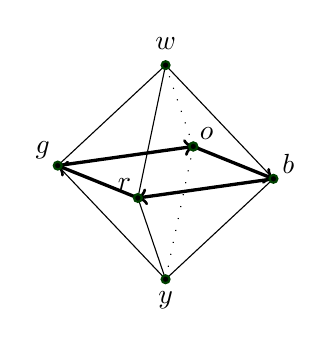
\begin{tikzpicture}%
  [x={(-0.860769cm, -0.121512cm)},
  y={(0.508996cm, -0.205391cm)},
  z={(-0.000053cm, 0.971107cm)},
  scale=1,
  eqback/.style={->, very thick},
  back/.style={loosely dotted, thin},
  eqedge/.style={->, very thick},
  edge/.style={black, thin},
  facet/.style={fill=blue!95!black,fill opacity=0.0},
  vertex/.style={inner sep=1pt,circle,draw=green!25!black,fill=black,thick}]
\coordinate (-1, -1, 0) at (-1, -1, 0);
\coordinate (-1, 1, 0) at (-1, 1, 0);
\coordinate (0, 0, -1) at (0, 0, -1);
\coordinate (0, 0, 1) at (0, 0, 1);
\coordinate (1, -1, 0) at (1, -1, 0);
\coordinate (1, 1, 0) at (1, 1, 0);
%% Drawing edges in the back
%%
\draw[edge,eqback] (-1, -1, 0) -- (-1, 1, 0);
\draw[edge,back] (-1, -1, 0) -- (0, 0, -1.4);
\draw[edge,back] (-1, -1, 0) -- (0, 0, 1.4);
\draw[edge,eqback] (1, -1, 0) -- (-1, -1, 0);
%% Drawing vertices in the back
%%
\node[vertex] at (-1, -1, 0)     {};
%% Drawing the facets
%%
\fill[facet] (1, 1, 0) -- (0, 0, -1.4) -- (1, -1, 0) -- cycle {};
\fill[facet] (1, 1, 0) -- (0, 0, 1.4) -- (1, -1, 0) -- cycle {};
\fill[facet] (1, 1, 0) -- (-1, 1, 0) -- (0, 0, 1.4) -- cycle {};
\fill[facet] (1, 1, 0) -- (-1, 1, 0) -- (0, 0, -1.4) -- cycle {};
%% Drawing edges in the front
%%
\draw[edge] (-1, 1, 0) -- (0, 0, -1.4);
\draw[edge] (-1, 1, 0) -- (0, 0, 1.4);
\draw[eqedge] (-1, 1, 0) -- (1, 1, 0);
\draw[edge] (0, 0, -1.4) -- (1, -1, 0);
\draw[edge] (0, 0, -1.4) -- (1, 1, 0);
\draw[edge] (0, 0, 1.4) -- (1, -1, 0);
\draw[edge] (0, 0, 1.4) -- (1, 1, 0);
\draw[eqedge] (1, 1, 0) -- (1, -1, 0);
%% Drawing the vertices in the front
%%
\begin{scope}[nodes=vertex]
\node[label=above right:\( b \)] at (-1, 1, 0)     {};
\node[label=below:\( y \)] at (0, 0, -1.4)     {};
\node[label=above:\( w \)] at (0, 0, 1.4)     {};
\node[label=above left:\( g \)] at (1, -1, 0)     {};
\node[label=above left:\( r \)] at (1, 1, 0)     {};
\node[label=above right:\( o \)] at (-1, -1, 0)     {};
\end{scope}
\end{tikzpicture}

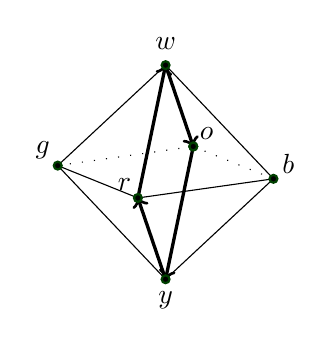
\begin{tikzpicture}%
  [x={(-0.860769cm, -0.121512cm)},
  y={(0.508996cm, -0.205391cm)},
  z={(-0.000053cm, 0.971107cm)},
  scale=1,
  eqback/.style={->, very thick},
  back/.style={loosely dotted, thin},
  eqedge/.style={->, very thick},
  edge/.style={black, thin},
  facet/.style={fill=blue!95!black,fill opacity=0.0},
  vertex/.style={inner sep=1pt,circle,draw=green!25!black,fill=black,thick}]
\coordinate (-1, -1, 0) at (-1, -1, 0);
\coordinate (-1, 1, 0) at (-1, 1, 0);
\coordinate (0, 0, -1) at (0, 0, -1);
\coordinate (0, 0, 1) at (0, 0, 1);
\coordinate (1, -1, 0) at (1, -1, 0);
\coordinate (1, 1, 0) at (1, 1, 0);
%% Drawing edges in the back
%%
\draw[edge,back] (-1, -1, 0) -- (-1, 1, 0);
\draw[edge,eqback] (-1, -1, 0) -- (0, 0, -1.4);
\draw[edge,eqback] (0, 0, 1.4) -- (-1, -1, 0);
\draw[edge,back] (1, -1, 0) -- (-1, -1, 0);
%% Drawing vertices in the back
%%
\node[vertex] at (-1, -1, 0)     {};
%% Drawing the facets
%%
\fill[facet] (1, 1, 0) -- (0, 0, -1.4) -- (1, -1, 0) -- cycle {};
\fill[facet] (1, 1, 0) -- (0, 0, 1.4) -- (1, -1, 0) -- cycle {};
\fill[facet] (1, 1, 0) -- (-1, 1, 0) -- (0, 0, 1.4) -- cycle {};
\fill[facet] (1, 1, 0) -- (-1, 1, 0) -- (0, 0, -1.4) -- cycle {};
%% Drawing edges in the front
%%
\draw[edge] (-1, 1, 0) -- (0, 0, -1.4);
\draw[edge] (-1, 1, 0) -- (0, 0, 1.4);
\draw[edge] (-1, 1, 0) -- (1, 1, 0);
\draw[edge] (0, 0, -1.4) -- (1, -1, 0);
\draw[eqedge] (0, 0, -1.4) -- (1, 1, 0);
\draw[edge] (0, 0, 1.4) -- (1, -1, 0);
\draw[eqedge] (1, 1, 0) -- (0, 0, 1.4) ;
\draw[edge] (1, 1, 0) -- (1, -1, 0);
%% Drawing the vertices in the front
%%
\begin{scope}[nodes=vertex]
\node[label=above right:\( b \)] at (-1, 1, 0)     {};
\node[label=below:\( y \)] at (0, 0, -1.4)     {};
\node[label=above:\( w \)] at (0, 0, 1.4)     {};
\node[label=above left:\( g \)] at (1, -1, 0)     {};
\node[label=above left:\( r \)] at (1, 1, 0)     {};
\node[label=above right:\( o \)] at (-1, -1, 0)     {};
\end{scope}
\end{tikzpicture}

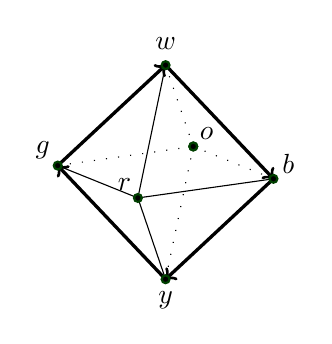
\begin{tikzpicture}%
  [x={(-0.860769cm, -0.121512cm)},
  y={(0.508996cm, -0.205391cm)},
  z={(-0.000053cm, 0.971107cm)},
  scale=1,
  eqback/.style={->, very thick},
  back/.style={loosely dotted, thin},
  eqedge/.style={->, very thick},
  edge/.style={black, thin},
  facet/.style={fill=blue!95!black,fill opacity=0.0},
  vertex/.style={inner sep=1pt,circle,draw=green!25!black,fill=black,thick}]
\coordinate (-1, -1, 0) at (-1, -1, 0);
\coordinate (-1, 1, 0) at (-1, 1, 0);
\coordinate (0, 0, -1) at (0, 0, -1);
\coordinate (0, 0, 1) at (0, 0, 1);
\coordinate (1, -1, 0) at (1, -1, 0);
\coordinate (1, 1, 0) at (1, 1, 0);
%% Drawing edges in the back
%%
\draw[edge,back] (-1, -1, 0) -- (-1, 1, 0);
\draw[edge,back] (-1, -1, 0) -- (0, 0, -1.4);
\draw[edge,back] (-1, -1, 0) -- (0, 0, 1.4);
\draw[edge,back] (1, -1, 0) -- (-1, -1, 0);
%% Drawing vertices in the back
%%
\node[vertex] at (-1, -1, 0)     {};
%% Drawing the facets
%%
\fill[facet] (1, 1, 0) -- (0, 0, -1.4) -- (1, -1, 0) -- cycle {};
\fill[facet] (1, 1, 0) -- (0, 0, 1.4) -- (1, -1, 0) -- cycle {};
\fill[facet] (1, 1, 0) -- (-1, 1, 0) -- (0, 0, 1.4) -- cycle {};
\fill[facet] (1, 1, 0) -- (-1, 1, 0) -- (0, 0, -1.4) -- cycle {};
%% Drawing edges in the front
%%
\draw[eqedge] (-1, 1, 0) -- (0, 0, -1.4);
\draw[eqedge] (0, 0, 1.4) -- (-1, 1, 0);
\draw[edge] (-1, 1, 0) -- (1, 1, 0);
\draw[eqedge] (0, 0, -1.4) -- (1, -1, 0);
\draw[edge] (0, 0, -1.4) -- (1, 1, 0);
\draw[eqedge] (1, -1, 0) -- (0, 0, 1.4);
\draw[edge] (0, 0, 1.4) -- (1, 1, 0);
\draw[edge] (1, 1, 0) -- (1, -1, 0);
%% Drawing the vertices in the front
%%
\begin{scope}[nodes=vertex]
\node[label=above right:\( b \)] at (-1, 1, 0)     {};
\node[label=below:\( y \)] at (0, 0, -1.4)     {};
\node[label=above:\( w \)] at (0, 0, 1.4)     {};
\node[label=above left:\( g \)] at (1, -1, 0)     {};
\node[label=above left:\( r \)] at (1, 1, 0)     {};
\node[label=above right:\( o \)] at (-1, -1, 0)     {};
\end{scope}
\end{tikzpicture}
\caption{The equators for \( w, b, r \).}
\end{figure}
\caption{\( \link \) for the vertices \( w, b\) and \( r \).}
\label{fig:triangle_of_equators}
\end{figure}

To extend \( T_0 \) to a function \( T_1 \) on the 1-skeleton we have complete freedom. Defining a map by induction makes clear that the action on paths is its own structure. Two functions on the octahedron could agree on points but differ on edges. We are going to identify this 1-dimensional freedom with a connection:

Continuing the example, we will do something ``tangent bundley'', imagining how \( T_1 \) changes as we slide from point to point in the embedding shown in the figures. Sliding from \( w \) to \( b \) and tipping the link as we go, we see \( r\mapsto r \) and \( o\mapsto o \) because those lie on the axis of rotation. Then \( g\mapsto w \) and \( b\mapsto y \). 

\begin{mydef}
Define \( T_1:\oo_1\to\EMzo \) on just the 1-skeleton by extending \( T_0 \) as follows:
Transport away from \( w \):
\begin{itemize}
\item \( T_1(wb):[b, r, g, o]\mapsto [y, r, w, o] \) (\( r, o \) fixed)
\item \( T_1(wr):[b, r, g, o]\mapsto [b, y, g, w] \) (\( b, g \) fixed)
\item \( T_1(wg):[b, r, g, o]\mapsto [w, r, y, o] \)
\item \( T_1(wo):[b, r, g, o]\mapsto [b, w, g, y] \)
\end{itemize}
Transport away from \( y \):
\begin{itemize}
\item \( T_1(yb):[b, o, g, r]\mapsto [w, o, y, r] \)
\item \( T_1(yr):[b, o, g, r]\mapsto [b, y, g, w] \)
\item \( T_1(yg):[b, o, g, r]\mapsto [y, o, w, r] \)
\item \( T_1(yo):[b, o, g, r]\mapsto [b, w, g, y] \)
\end{itemize}
Transport along the equator:
\begin{itemize}
\item \( T_1(br):[w, o, y, r]\mapsto [w, b, y, g] \) 
\item \( T_1(rg):[w, b, y, g]\mapsto [w, r, y, o] \)
\item \( T_1(go):[w, r, y, o]\mapsto [w, g, y, b] \)
\item \( T_1(ob):[w, g, y, b]\mapsto [w, o, y, r] \)
\end{itemize}
\end{mydef}

It's very important to be able to visualize what \( T_1 \) does to triangular paths such as \( wb\cdot br\cdot rw \) (which circulates around the boundary of face \( wbr \)). You can see it if you imagine Figure~\ref{fig:triangle_of_equators} as the frames of a short movie. Or you can place your palm over the top of a cube and note where your fingers are pointing, then slide your hand to an equatorial face, then along the equator, then back to the top. The answer is: you come back rotated clockwise by a quarter-turn. 

\begin{mydef}
\label{def:octahedron_holonomy}
The map \( R:C_4\to C_4 \) rotates by one quarter turn, one ``click":
\begin{multicols}{2}
\begin{itemize}
\item \( R(c_1) = c_2 \)
\item \( R(c_2) = c_3 \)
\item \( R(c_3) = c_4 \)
\item \( R(c_4) = c_1 \)
\item \( R(c_1c_2) = c_2c_3 \)
\item \( R(c_2c_3) = c_3c_4 \)
\item \( R(c_3c_4) = c_4c_1 \)
\item \( R(c_4c_1) = c_1c_2 \)
\end{itemize}
\end{multicols}
\end{mydef}

Note by univalence the equivalence \( R \) gives a loop in the universe, a term of \( C_4=_{\EMzo}C_4 \).

Now let's extend \( T_1 \) to all of \( \oo \) by providing values for the eight faces. The face \( wbr \) is a path from \( \refl_w \) to the concatenation \( wb\cdot br\cdot rw \), and so the image of \( wbr \) under the extended version of \( T_1 \) must be a homotopy from \( \refl_{T_1(w)} \) to \( T_1(wb\cdot br\cdot rw) \). Here \emph{there is no additional freedom}.

\begin{mydef}
\label{def:octahedron_curvature}
Define \( T_2:\oo\to\EMzo \) by extending \( T_1 \) to the faces as follows:
\begin{multicols}{2}
\begin{itemize}
\item \( T_2(wbr)=H_R \) 
\item \( T_2(wrg)=H_R \)
\item \( T_2(wgo)=H_R \)
\item \( T_2(ybo)=H_R \)
\item \( T_2(yrb)=H_R \) 
\item \( T_2(ygr)=H_R \)
\item \( T_2(yog)=H_R \)
\item \( T_2(ybo)=H_R \)
\end{itemize}
\end{multicols}
where \( H_R:R=\refl_{C_4} \) is the obvious homotopy given by composition with \( R^{-1} \). Passing through univalence we get a 2-path between \( R \) and \( \refl \) in the loop space \( C_4=_{\EMzo}C_4 \).
\end{mydef}

\subsection{Existence of connections}

How confident can we be that we can always define a connection on an arbitrary combinatorial manifold? Two things make the octahedron example special: the link is a 4-gon at every vertex, and every edge extends to a symmetry of the entire octahedron, embedded in 3-dimensional space. This imposed a coherence on the interactions of all the choices we made for the connection, which we can worry may not exist for more complex combinatorial data.

We know as a fact outside of HoTT that any combinatorial surface that has been realized as a triangulated surface embedded in 3-dimensional euclidean space can inherit the parallel transport entailed in the embedding. We could then approximate that data to arbitrary precision with enough subdivision of the fibers of \( T \).

What would a proof inside of HoTT look like? We will leave this as an open question.



\section{Leibniz, Gauss-Bonnet, Poincaré-Hopf}

\subsection{The Leibniz (product) rule}

This is a slight aside in the context of this note, but it belongs here anyway because it follows from the slogan ``\( \ap \) is \( d \)'', i.e. that calculus and differential geometry are visible in type theory through the action on paths, which is a finite version of the infinitesimal tangent vector. If we think we have some new understanding of the operator \( d \), then we should test it by finding the Leibniz rule.

The Leibniz rule for exterior differentiation states that if \( f, g:M\to \rr \) are two smooth functions to the real numbers then \( d(fg) = fdg + gdf \). Here \( fg \) is the function formed by taking the pointwise product of \( f \) and \( g \). This is an interaction between multiplication in \( \rr \) and the action on vectors of smooth functions (the 1-forms \( df \) and \( dg \)). 

To examine this situation in HoTT we need type-theoretic functions \( f, g:M\to B \) from some type \( M \) to a central H-space \( B \). Let \( \mu:B\to B\to B \) be the H-space multiplication. How does \( \mu \) act on paths? Suppose we have \( a, a', b, b':B \) and \( p:a=_B a', q:b=_B b' \). Then we also have homotopies \( \mu(p, -):\mu(a, -)=_{B\to B}\mu(a', -) \) and \( \mu(-,q):\mu(-,b)=_{B\to B}\mu(-,b'). \) Since \( \mu(a, -):B=B \) is an (unpointed) equivalence of \( B \), and similarly for \( \mu(b, -) \) and so on, this data assembles into the following diagram of higher groupoid morphisms:

\begin{center}
% https://q.uiver.app/#q=WzAsMyxbMiwwLCJCIl0sWzAsMCwiQiJdLFs0LDAsIkIiXSxbMSwwLCJcXG11KGEsLSkiLDAseyJjdXJ2ZSI6LTN9XSxbMSwwLCJcXG11KGEnLC0pIiwyLHsiY3VydmUiOjN9XSxbMCwyLCJcXG11KC0sYikiLDAseyJjdXJ2ZSI6LTN9XSxbMCwyLCJcXG11KC0sYicpIiwyLHsiY3VydmUiOjN9XSxbMyw0LCJcXG11KHAsLSkiLDIseyJzaG9ydGVuIjp7InNvdXJjZSI6MjAsInRhcmdldCI6MjB9fV0sWzUsNiwiXFxtdSgtLHEpIiwyLHsic2hvcnRlbiI6eyJzb3VyY2UiOjIwLCJ0YXJnZXQiOjIwfX1dXQ==
\begin{tikzcd}
  B && B && B
  \arrow[""{name=0, anchor=center, inner sep=0}, "{\mu(a,-)}", curve={height=-18pt}, from=1-1, to=1-3]
  \arrow[""{name=1, anchor=center, inner sep=0}, "{\mu(a',-)}"', curve={height=18pt}, from=1-1, to=1-3]
  \arrow[""{name=2, anchor=center, inner sep=0}, "{\mu(-,b)}", curve={height=-18pt}, from=1-3, to=1-5]
  \arrow[""{name=3, anchor=center, inner sep=0}, "{\mu(-,b')}"', curve={height=18pt}, from=1-3, to=1-5]
  \arrow["{\mu(p,-)}"', shorten <=5pt, shorten >=5pt, Rightarrow, from=0, to=1]
  \arrow["{\mu(-,q)}"', shorten <=5pt, shorten >=5pt, Rightarrow, from=2, to=3]
\end{tikzcd}
\end{center}

And so the two homotopies can be horizontally composed to give a path \[ \mu(p,-)\star\mu(-,q): \mu(a, b)=\mu(a',b'). \] Horizontal composition is given by \[\mu(p,-)\star\mu(-,q)\defeq(\mu(p,-)\cdot_r \mu(-,b))\cdot(\mu(a', -)\cdot_l\mu(-, q))\] where \[ \mu(p,-)\cdot_r\mu(-,b):\mu(a,b)=\mu(a',b) \] and \[ \mu(a',-)\cdot_l\mu(-,q):\mu(a',b)=\mu(a',b') \] are defined by path induction.  See the HoTT book Theorem 2.1.6 on the Eckmann-Hilton argument\cite{hottbook}.

We can recognize the process of using whiskering to form horizontal composition in the Leibniz rule. 

Quick aside: moving from infinitesimal calculus to finite groupoid algebra actually involves two changes. The first is the change from vectors to paths, forms to functions and so on. But it's also the case that tangent vectors have just the one basepoint, whereas paths have two endpoints. You can see this play out in this example, where \( a \) and \( a' \) were distinct points (and \( b \) and \( b' \)).

The horizontal composition we build lives entirely in \( B \) and we didn't make use of \( M \) yet. The Leibniz rule will be a pointwise version of what's going on in \( B \). Denote by \( \mu\circ(f,g):M\to B \) the map which sends \( x\mapsto \mu(f(x),g(x)) \).

\begin{mylemma}
Given \( f, g:M\to B \) and \( p:x=_M y \) then 
\begin{align*}
 \ap(\mu\circ(f,g))(p)&=\mu(f(p),-)\star\mu(-,g(p))\\
 &=\left[\mu(f(p),-)\cdot_r \mu(-,g(x))\right]\cdot \left[\mu(f(y),-)\cdot_l\mu(-,g(p))\right]\\
 &:\mu(f(x),g(x))=\mu(f(y),g(y))
\end{align*}
\end{mylemma}

\subsection{The total curvature}

\begin{mydef}
Let \( F(M) \) denote the groupoid of faces of \( M \) generated by the faces in its constructor. Let \( V:\pit{f:F(M)}f \) be a selected vertex of every face, and let \( \partial:\pit{f:F(M)}Vf=_M Vf \) be the clockwise boundary path around a face. Let \( v \) be the basepoint of \( M \). Then in particular we have \( M:F(M) \) the concatenation of all faces (i.e. \( M \) itself), and we have \( \partial(M):v=_M v \) which is the concatenation of all boundaries.
\end{mydef}

Observe that each generating edge of \( M \) is visited once in each direction in the concatenation \( \partial(M) \). 

The bundle map \( T \) can be examined on each face. On a face \( f \) bounding a loop \( \ell:v=_M v \) the map \( T:M\to\EMzo \) assigns a homotopy \( T(f):\refl_v=T(\ell) \), where \( T(\ell) \) is an automorphism of \( T(v) \). On the composition of all faces we have \( T(M):T(v)=T(v) \), the \defemph{total curvature}.

It is crucial that \( T(M) \) can be nontrivial (i.e. not \( \refl_v \)) even though it's computed by transporting across every edge in \( \partial(M) \) once in each direction!

\subsection{The total index}

If we have \( M\setminus Z \) for some isolated set of verticies \( Z \), then for each \( z:Z \) we can compose all the faces which contain \( z \), forming a new face. In this way we produce an equivalent type \( M_Z\simeq M \) but which is no longer combinatorial since we have erased some of the edges from some of the neighborhoods. See Figure~\ref{fig:torus_morse} where the outlined hexagons are the composition of the six triangular faces around a zero.

If \( X \) is a vector field with isolated zeros on \( Z \), then \( M_Z \) is a convenient replacement for \( M \) because \( X \) is a partial function defined on all of \( M_Z \) except for a collection of faces, each of which bounds one of the zeros of \( Z \).

\begin{mynote}
If the combinatorial manifold was imported into type theory via some process of sampling or other, perhpaps more theoretical, construction then we should allow for zeros to occur on verticies, edges, or faces. We can reduce the case of a zero on a vertex or edge to that of a face with the replacement method just described. The original combinatorial neighborhood structure continues to live in the fibers of \( T \), it's only the base manifold that has been replaced.
\end{mynote}

\begin{mydef}
Given a face \( f:F(M\setminus Z) \), define \defemph{the index of \( X \) on \( f \)} to be the winding number (also called the degree) of \( X(\partial f) \). The \defemph{total index} of \( X \) on \( M\setminus Z \) is the index of \( X \) on \( \partial(M\setminus Z) \).
\end{mydef}

The index computation skips some faces of \( M \) and can most definitely be nonzero.

\subsection{Equality of total index and total curvature}

Here we closely follow the classical proof of Hopf\cite{hopf}, presented in detail in Needham\cite{needham}.

\begin{mythm}
The total curvature's winding number is equal to the total index of \( X \).
\end{mythm}
The fact that the index was already an integer, whereas the curvature is a path accounts for the factor of \( 2\pi \) in some classical statement of this theorem (e.g. \cite{needham} section 26.3).
\begin{proof}
Let \( C \) be a fixed pointed polygon (e.g. \( C_4 \) or \( C_6 \) which we met earlier). We can consider \( X \) to map each vertex of \( M_Z \) to \( C \). On each face of \( M_Z \) (no faces are omitted) we traverse the boundary, which is in the domain of both \( T \) and of \( X \). So we avoid the complication that \( X \) is not defined on some of the faces by remaining on the 1-skeleton. For a given edge \( e_{12}:v_1=_{M_Z} v_2 \) the function \( \tr_{e_{12}}X(v_1)=X(v_2) \) is a path in \( C \). We will traverse every edge twice, once in each direction, which will cancel to give \( \refl_v \). In particular the boundaries around the zeros of \( X \) are themselves traversed twice in opposite directions, canceling the total index.
\end{proof}

\begin{mycor}
The total index of a vector field with isolated zeros is independent of the vector field.
\end{mycor}

\begin{mycor}
The total curvature is an integer.
\end{mycor}

The last step is to link this value to the Euler characteristic.

\subsection{Identification with Euler characteristic}

Combinatorial manifolds are intuitive objects that connect directly to the classical definition of Euler characteristic. We can argue using Morse theory, the study of smooth real-valued functions on smooth manifolds and their singularities. Classically the gradient of a Morse function is a vector field that can be used to decompose the manifold into its \emph{handlebody decomposition}. This would be an excellent story to pursue in future work.

Imagine a combinatorial manifold of a genus g oriented surface standing upright with the holes forming a vertical sequence. Now install a vector field that points downward whenever possible. This vector field will have a zero at the top and bottom, and one at the top and bottom of each hole. The top and bottom will be index 1, and ones around the holes will be index -1. We include some sketches in the case of a torus. This illustrates how we obtain the formula for genus \( g \): \( \chi(M)=2-2g \).

\begin{figure}[htbp]
\centering
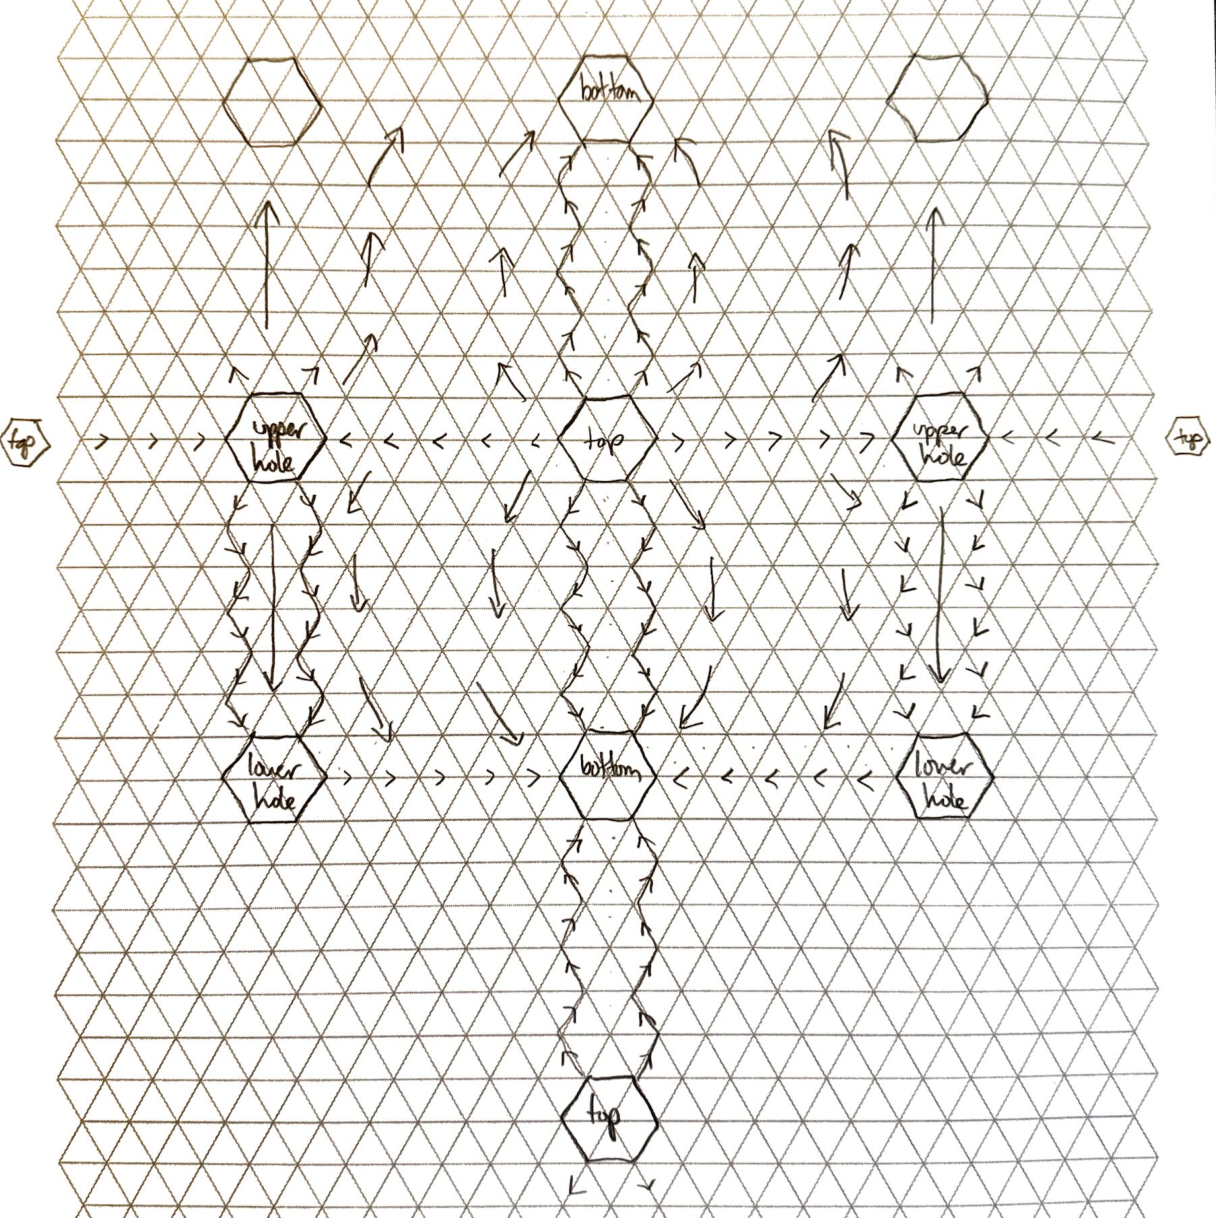
\includegraphics[width=400pt]{torus_morse_grad.pdf}
\caption{A sketch of downward flow on the torus.}
\label{fig:torus_morse}
\end{figure}

\begin{figure}[htbp]
\centering
% https://q.uiver.app/#q=WzAsOCxbMCwwLCJcXGJ1bGxldCJdLFswLDEsIlxcYnVsbGV0Il0sWzAsMiwiXFxidWxsZXQiXSxbMCwzLCJcXGJ1bGxldCJdLFsxLDAsIlxcbWF0aHJte3RvcH0iXSxbMSwxLCJcXG1hdGhybXt1cHBlclxcIGhvbGV9Il0sWzEsMiwiXFxtYXRocm17bG93ZXJcXCBob2xlfSJdLFsxLDMsIlxcbWF0aHJte2JvdHRvbX0iXSxbMCwxLCIiLDIseyJjdXJ2ZSI6LTEsInN0eWxlIjp7ImJvZHkiOnsibmFtZSI6ImRhc2hlZCJ9fX1dLFswLDEsIiIsMCx7ImN1cnZlIjoxLCJzdHlsZSI6eyJib2R5Ijp7Im5hbWUiOiJkYXNoZWQifX19XSxbMiwzLCIiLDAseyJjdXJ2ZSI6LTEsInN0eWxlIjp7ImJvZHkiOnsibmFtZSI6ImRhc2hlZCJ9fX1dLFsyLDMsIiIsMix7ImN1cnZlIjoxLCJzdHlsZSI6eyJib2R5Ijp7Im5hbWUiOiJkYXNoZWQifX19XSxbMCwzLCIiLDEseyJjdXJ2ZSI6LTV9XSxbMCwzLCIiLDEseyJjdXJ2ZSI6NX1dLFsxLDIsIiIsMSx7ImN1cnZlIjoyfV0sWzEsMiwiIiwxLHsiY3VydmUiOi0yfV1d
\begin{tikzcd}[cramped]
  \bullet & {\mathrm{top}} \\
  \bullet & {\mathrm{upper\ hole}} \\
  \bullet & {\mathrm{lower\ hole}} \\
  \bullet & {\mathrm{bottom}}
  \arrow[curve={height=-6pt}, dashed, from=1-1, to=2-1]
  \arrow[curve={height=6pt}, dashed, from=1-1, to=2-1]
  \arrow[curve={height=-30pt}, from=1-1, to=4-1]
  \arrow[curve={height=30pt}, from=1-1, to=4-1]
  \arrow[curve={height=12pt}, from=2-1, to=3-1]
  \arrow[curve={height=-12pt}, from=2-1, to=3-1]
  \arrow[curve={height=-6pt}, dashed, from=3-1, to=4-1]
  \arrow[curve={height=6pt}, dashed, from=3-1, to=4-1]
\end{tikzcd}
\caption{Schematic of the zeros of the downward flow of a torus.}
\label{fig:torus_morse_skel}
\end{figure}


\bibliography{connections}
\end{document}



